\documentclass[twocolumn, letterpaper,13pt]{scrartcl}

\usepackage{uog_factsheet}
\usepackage{xcolor}
\usepackage{hyperref}

\definecolor{seablue}{RGB}{0,127,169}

\begin{document}
    \title{\color{seablue}Data Visualization Evaluation protocol for a web page displaying a Choropleth map}

	\maketitle
	
    \section*{Introduction}
    
    The following proposes an evaluation protocol to assess the usability of a Data Visualization application processing data from the deep learning WASABI dataset.
    \newline
    The application is a web page displaying a Choropleth map, coded in Javascript, that is available on Github\footnote{\href{https://github.com/LMquentinLR/choropleth\_wasabi\_dataset}{Link to github}}.
    \newline
    This document must not be shared with any participant as no before-hand knowledge of what they will be using is permitted. The goal is to avoid participants having prepared for the evaluation task.
    \newline
    \newline
    The whole process is structured in three steps:
    \begin{itemize}
        \item Welcoming, briefing, and pre-interview of participants
        \item Assignment to be completed by the kept participants
        \item Survey completion by the participants and debriefing \& final interview
    \end{itemize}
    
    \section*{Evaluation Format}

    \subsection*{participant-Oriented Evaluation Method}
    
    We choose a participant-oriented method conducted with real-participants. The experimental question is: 
    
    \begin{quote}
        Can a participant complete a set of increasingly demanding tasks on a data visualization format they have never seen before?
    \end{quote}
    
    We focus on efficiency (how quickly they can achieve a task) and participant satisfaction (of their experience).

    \subsection*{Hypothesis Regarding The Data Visualization Format}
 
    The experimental design is not duplicated between various types of UI or between different conditions. As such, there are no hypotheses associated with the current implementation of a data visualization. 
 
    \subsection*{Metrics}
    
    To measure the independent reaction of participants to the content, the following metrics are used:
    
    \begin{itemize}
        \item Number of successful completions of a task (effectiveness)
        \item Number of clicks to achieve a task compared to the minimum number of clicks possible (effectiveness)
        \item Time spent between the start of the task and its completion (effectiveness)
        \item Tracking of eye movements (effectiveness)
        \item Tracking of mouse pointer movements (effectiveness)
        \item end-questionnaire to assess usability
    \end{itemize}
    
    \section*{Test Session Checklist}
    A session corresponds to running a single participant through the whole process from start to finish, unless a stopping event is reached. Any session \textbf{must} follow the following steps:
    \begin{itemize}
        \item Welcome the participant and introduce them to each involved party: the tester/observer, etc.
        \item Introduce the participant to:
        \begin{itemize}
            \item the evaluation process and its context: reason for evaluation participants on the task, and goal of compiling the data
            \item the setting: They will be using a Data Visualization App displayed on a web browser
            \item the place: the testing area
            \item the hardware setup: computer monitor (output to the participant), mouse (input from the participant), camera (mean of observation of the participant), and recorder (for the screen displayed on the computer monitor)
        \end{itemize}
        \item Ask the participant if they have any questions, are comfortable, and wish to proceed
        \item Have the participant sign any disclosure agreement or letter of understanding of what their participation entails
        \item Ask the participant if they have any questions, are comfortable, and wish to proceed
        \item Have the participant answer a profile questionnaire (Pre-Task)
        \item Ask the participant if they have any questions, are comfortable, and wish to proceed
        \item If so, the tester/observer removes themselves from the test area, and mentioned the go to the participant
        \item The participant may obtain/reveal their instructions and proceed
        \item Once each task is performed, the tester/observer comes back to the test area
        \item Ask the participant if they have any questions, are comfortable, and wish to proceed
        \item Have the participant answer a post-task questionnaire
        \item Thank the participant as they leave
    \end{itemize}
    
    \section*{Pre-Task Questionnaire}
    
    During the initial part of the test session, the participant will be offered to complete a questionnaire once a disclosure agreement/letter of understanding has been signed. The questionnaire is set in two parts. 
    \begin{itemize}
        \item Participant information: Name, contact information, etc. which make the participant reachable
        \item participant experience (meant to help size the participant's profile):
        \begin{itemize}
            \item Do you play a music instrument? [Y]/[N]
            \item Are you subscribed to an audio streaming platform? [Y]/[N]
            \item How many hours per week do you dedicate to listening to music? [less than 1 hour]/[1 to 5h]/[6 to 10h]/[More than 10 hours]
            \item How many music genres do you say you mainly listen to? [1]/[2]/[3]/[More than 3]
            \item Do you read or follow (on social media) music bands or news media dedicated to music (e.g. Rolling Stones magazine)? [Y]/[N]
        \end{itemize}
    \end{itemize}
    
    \section*{Tasks}
    
    Once the checklist is done and the participant is ready to start the session, they will be given a series of task to perform.

    \subsubsection*{Task 1}
    \begin{itemize}
        \item \textbf{Instruction:} You have entered a new website displaying a world map. Find the average population for the United States of America in the 2000s.
        \item \textbf{Evaluation:} On a scale from 1 (least) to 5 (very), how easy was it to find the value?
        \item \textbf{Follow-up Question:} What would you change to the process to make it easier?
    \end{itemize}
    
    \subsubsection*{Task 2}
    \begin{itemize}
        \item \textbf{Instruction:} Find the number of rock bands in the United States in the 1980s.
        \item \textbf{Evaluation:} On a scale from 1 (least) to 5 (very), how easy was it to find the value?
        \item \textbf{Follow-up Question:} What would you change to the process to make it easier?
    \end{itemize}
    
    \subsubsection*{Task 3}
    \begin{itemize}
        \item \textbf{Instruction:} Find the ratio of rock bands per one million people in the United States in the 1960s.
        \item \textbf{Evaluation:} On a scale from 1 (least) to 5 (very), how easy was it to find the value?
        \item \textbf{Follow-up Question:} What would you change to the process to make it easier?
    \end{itemize}
    
    \subsubsection*{Task 4}
    \begin{itemize}
        \item \textbf{Instruction:} Find the ratio of electro bands in Germany in the 1990s.
        \item \textbf{Evaluation:} On a scale from 1 (least) to 5 (very), how easy was it to find the value?
        \item \textbf{Follow-up Question:} What would you change to the process to make it easier?
    \end{itemize}
    
    \subsubsection*{Task 5}
    \begin{itemize}
        \item \textbf{Instruction:} Find the percentage share of hip-hop bands over the total number of bands in France in the 1990s.
        \item \textbf{Evaluation:} On a scale from 1 (least) to 5 (very), how easy was it to find the value?
        \item \textbf{Follow-up Question:} What would you change to the process to make it easier?
    \end{itemize}
    
    \subsubsection*{Task 6}
    \begin{itemize}
        \item \textbf{Instruction:} Find whether Andorra (a small country between France and Spain) had metal bands in the 2000s.
        \item \textbf{Evaluation:} On a scale from 1 (least) to 5 (very), how easy was it to find the answer?
        \item \textbf{Follow-up Question:} What would you change to the process to make it easier?
    \end{itemize}

    \subsubsection*{Task 7}
    \begin{itemize}
        \item \textbf{Instruction:} Find whether Andorra (a small country between France and Spain) had metal bands in the 2000s.
        \item \textbf{Evaluation:} On a scale from 1 (least) to 5 (very), how easy was it to find the value?
        \item \textbf{Follow-up Question:} What would you change to the process to make it easier?
    \end{itemize}
    
    \begin{figure}	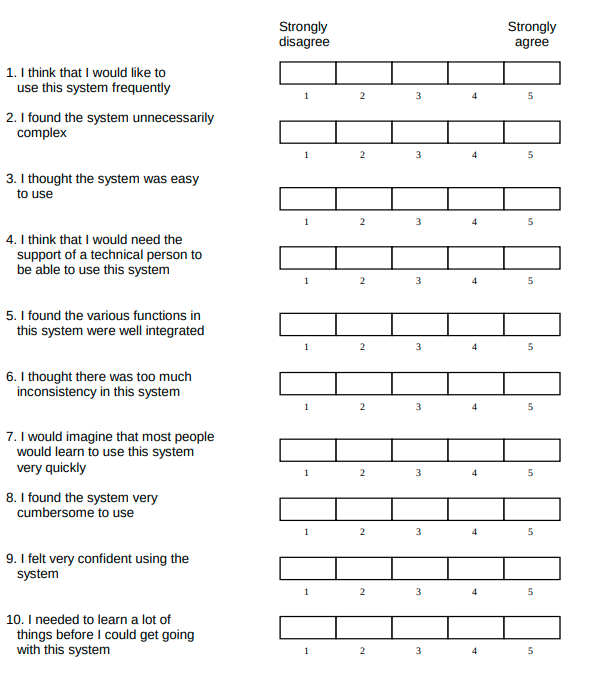
\includegraphics[width=0.98\linewidth]{SUS.png}
    \caption{Original System Usability Scale questionnaire\label{fig:a}}
    \end{figure}
    
    \subsubsection*{Task 8}
    \begin{itemize}
        \item \textbf{Instruction:} Find which country had the highest ratio of jazz band per capita in the world.
        \item \textbf{Evaluation:} On a scale from 1 (least) to 5 (very), how easy was it to find the value?
        \item \textbf{Follow-up Question:} What would you change to the process to make it easier?
    \end{itemize}

    \subsubsection*{Task 9}
    \begin{itemize}
        \item \textbf{Instruction:} Automatically play the sequence of map per decade for the genre Punk.
        \item \textbf{Evaluation:} On a scale from 1 (least) to 5 (very), how easy was it to find the value?
        \item \textbf{Follow-up Question:} What would you change to the process to make it easier?
    \end{itemize}
    
    \section*{End-Questionnaire}
    
    The end questionnaire will follow the System Usability Scale standard (see Fig. \ref{fig:a}) from J. Brooke\cite{brook}. It standard questionnaire used for assessing overall usability of a system/tool/etc.
    
    Based on 10 standard questions, it allows to calculate a score from 0 to 100 (from worst to best) to inform testers/observers of the overall usability and efficient learning of a system/tool/etc. by a novice user.
    
    \bibliographystyle{unsrtnat}   
    \begin{thebibliography}{9}

    \bibitem{brook}
    Brooke, John. (1995). \textit{\href{https://hell.meiert.org/core/pdf/sus.pdf}{SUS: A quick and dirty usability scale. Usability}} Eval. Ind.. 189. 

    \end{thebibliography}
    
\end{document}